\documentclass{article}

\usepackage[utf8]{inputenc}
\usepackage[spanish]{babel}

\usepackage{geometry}               % Márgenes del documento
\usepackage{amsfonts}
\usepackage{graphicx}

\usepackage{tabularx}

\usepackage{amsthm} % para teoremas y lemas

\usepackage[nottoc]{tocbibind}

\usepackage{color}
\usepackage[pdftex, colorlinks=true, linkcolor=blue, urlcolor=red, filecolor=magenta, citecolor=green]{hyperref}
\definecolor{gray97}{gray}{.97}
\definecolor{gray75}{gray}{.75}
\definecolor{gray45}{gray}{.45}

\usepackage{listings}
\usepackage[usenames,dvipsnames]{xcolor}
\colorlet{keyword}{blue!100!black!80}
\colorlet{STD}{Lavender}
\colorlet{comment}{green!80!black!90}

\lstdefinestyle{xml}{
	language     = XML, %basicstyle=\ttfamily\footnotesize,
	morestring=[b]",
	moredelim=[s][\bfseries\color{Maroon}]{<}{\ },
	moredelim=[s][\bfseries\color{Maroon}]{</}{>},
	moredelim=[l][\bfseries\color{Maroon}]{/>},
	moredelim=[l][\bfseries\color{Maroon}]{>},
	morecomment=[s]{<?}{?>},
	morecomment=[s]{<!--}{-->},
	commentstyle=\color{comment},
	stringstyle=\color{blue},
	identifierstyle=\color{red},		
	showstringspaces=false,
	tabsize=3,
	numbers=left, % Donde se situan los numeros
	frame=single, % Se pone un marco
	backgroundcolor = \color{gray97},
	basicstyle   = \footnotesize \ttfamily,
	keywordstyle = [1]\color{keyword}\bfseries,
	keywordstyle = [2]\color{STD}\bfseries,
	breaklines=true                % sets automatic line breaking
}

\lstdefinestyle{sharpc}{
	language     = [Sharp]C,
	tabsize=3,
	numbers=left, % Donde se situan los numeros
	frame=single, % Se pone un marco
	backgroundcolor = \color{gray97},
	basicstyle   = \footnotesize \ttfamily,
	keywordstyle = [1]\color{keyword}\bfseries,
	keywordstyle = [2]\color{STD}\bfseries,
	breaklines=true,                % sets automatic line breaking
	commentstyle = \color{comment}
}

\geometry{a4paper}                  % Tamaño y márgenes del documento
\geometry{left=2.5cm,top=2.5cm}
\geometry{bottom=2.5cm,right=2.5cm}

\geometry{driver=dvips,pdftex} % ???
\setcounter{secnumdepth}{5}    % ???
\setcounter{tocdepth}{5}       % ???

%--------------------------------------------------------------------------
\title{\textbf{Integración de Sistemas} \\ Práctica .NET}
\author{
	Francisco Abel Cedrón Santaeufemia \\
	%\texttt{Informacion relevante} \\
	\texttt{$francisco.cedron@udc.es$}
	\and
	Nuria López Rivas \\
	\texttt{$nuria.lrivas@udc.es$}
	}
\date{} %Asi no inserta la fecha


\begin{document}


\maketitle % Pone titulo, autor

\renewcommand{\abstractname}{Abstract} % El nombre que aparece al principio del abstract
\begin{abstract}
	En el presente documento se expone la práctica desarrollada por Francisco Abel y Nuria que se corresponde con la aplicación Web propuesta en el enunciado de la práctica 2 de Integración de Sistemas, así como algunos aspectos a tener en cuenta sobre la implementación realizada.
\end{abstract}

\renewcommand{\contentsname}{} % Lo que pone en el indice
\tableofcontents

%\vspace{2cm} % Para dejar un espacio con respecto a la tabla
\newpage

\section{Arquitectura Global}

	En este apartado se comenta la estructura global de paquetes de la aplicación. A continuación se detallan los principales paquetes del proyecto, explicando brevemente lo que contienen:

\begin{itemize}
	\item \textbf{Model:} Proyecto correspondiente a la capa modelo del proyecto. Incluye las clases persistentes (autogeneradas a partir de las tablas de base de datos diseñada), además de los siguientes paquetes:
	
	\begin{itemize}
		\item \textbf{CommentDao}: Contiene la interfaz e implementación del DAO comentarios (clase persistente \emph{Comment}, consúltese el aparato \ref{cap:ClasesPersistentes} para ver las clases persistentes).
		\item \textbf{CommentService}: Contiene la interfaz e implementación del servicio dedicado a operaciones relacionadas con comentarios y sus etiquetas.
		\item \textbf{Exceptions}: Contiene algunas excepciones que se podrían dar en cualquier servicio o DAO (más concretamente contiene la clase \emph{EmptyStringException}).
		\item \textbf{FavouriteDao}: Contiene la interfaz e implemetación del Dao de productos favoritos (clase persistente \emph{Favourite}).
		\item \textbf{FavouriteService}: Contiene la interfaz e implementación del servicio dedicado a operaciones relacionadas con la gestión de los productos favoritos de cada usuario).
		\item \textbf{LabelDao}: Contiene la interfaz e implementación del DAO de etiquetas (clase persistente \emph{Label}).
		\item \textbf{ProductService}: Contiene la interfaz e implementación del servicio dedicado a las consultas sobre los productos \footnote{En esta primera iteración la implementación está vacía cuya una función es lanzar una excepción de clase no implementada.}.
		\item \textbf{UserProfileDao}: Contiene la interfaz e implementación del DAO de usuarios (clase persistente \emph{UserProfile}).
		\item \textbf{UserService}: Contiene la interfaz e implementación del servicio dedicado a las operaciones sobre usuarios. También incluye un subpaquete con excepciones lanzadas por métodos de este servicio y un subpaquete con clases de utilidad para este servicio como por ejemplo la clase \emph{PasswordEncrypter}.
		\item \textbf{ValuationDao}: Contiene la interfaz e implementación del DAO de valoración (clase persistente \emph{Valuation}).
		\item \textbf{ValuationService}: Contiene la interfaz e implementación del servicio dedicado a las valoraciones que realizan los usuarios.
	\end{itemize}
	
	\item \textbf{Test}: Proyecto de Test dedicado a las pruebas de integración de la capa modelo. Incluye una clase de test por cada servicio implementado en la capa modelo:
	
	\begin{itemize}
		\item \textbf{ICommentServiceTest.cs}: Clase con los métodos de pruebas para el servicio de comentarios.
		\item \textbf{IFavouriteServiceTest.cs}: Clase con los métodos de pruebas para el servicio de favoritos.
%		\item \textbf{IProductServiceTest.cs}: Clase con los métodos de pruebas para el servicio de productos.
		\item \textbf{IUserServiceTest.cs}: Clase con los métodos de pruebas para el servicio de usuarios.
		\item \textbf{IValuationServiceTest.cs}: Clase con los métodos de pruebas para el servicio de valoración.
	\end{itemize}
	
	\item \textbf{Web}: Proyecto correspondiente a la capa vista.

	\begin{itemize}
		\item \textbf{App\_GlobalResources}: Contiene recursos globales del proyecto web.
		\item \textbf{App\_LocalResources}: Contiene recursos locales de las páginas raíz del proyecto.
		\item \textbf{Css}: Contiene hojas de estilo \emph{css} utilizadas en la aplicación web.
		\item \textbf{HTTP}: Incluye clases con funcionalidades para la aplicación (como la gestión de usuarios).
		\item \textbf{ico}: Contiene el favicon de la applicación web.
		\item \textbf{img}: Contiene las imágenes.
		\item \textbf{js}: Incluye archivos javascript utilizados en la práctica.
		\item \textbf{Pages}: Incluye las páginas de contenido de la aplicación, así como los paquetes de recursos locales para cada sección.
		\begin{itemize}
			\item \textbf{App\_LocalResources}: Paquete con los recursos locales para las páginas del proyecto web incluidas en el paquete \emph{Pages}.
			\item \textbf{Comment}: Contiene las páginas y archivos locales para los casos de uso orientados al servicio de comentatios.
			\item \textbf{Product}: Contiene las páginas y archivos locales para los casos de uso orientados al servicio de productos.
			\item \textbf{Valuation}: Contiene las páginas y archivos locales para los casos de uso orientados a las valoraciones.
			\item \textbf{User}: Contiene las páginas con los casos de uso orientados al servicio de usuarios y grupos de usuario (como, por ejemplo, el registro o la autenticación de un usuario).
			\item \textbf{Errors}: Páginas de error personalizadas.
		\end{itemize}
		\item \textbf{XSLT}: Incluye los ficheros \emph{xslt} para convertir los datos de los productos.
	\end{itemize}			
\end{itemize}

	En la figura \ref{fig:ArquitecturaGlobal} se muestra la arquitectura global de paquetes de la aplicación mediante un diagrama de paquetes de UML.

\begin{figure}[h]
  \centering
    \includegraphics[width=0.85\textwidth]{img/arquitectura.pdf}
  \caption{Arquitectura global de paquetes de la aplicación.}
  \label{fig:ArquitecturaGlobal}
\end{figure}	

\section{Modelo}

	En esta sección se muestran los detalles de diseño e implementación de la capa modelo de la aplicación.

\subsection{Clases persistentes} \label{cap:ClasesPersistentes}

	En la figura \ref{fig:ClasesPersistentes}, se muestran todas las clases persistentes modeladas, así como las relaciones relevantes entre ellas.
	
\begin{figure}[h]
  \centering
    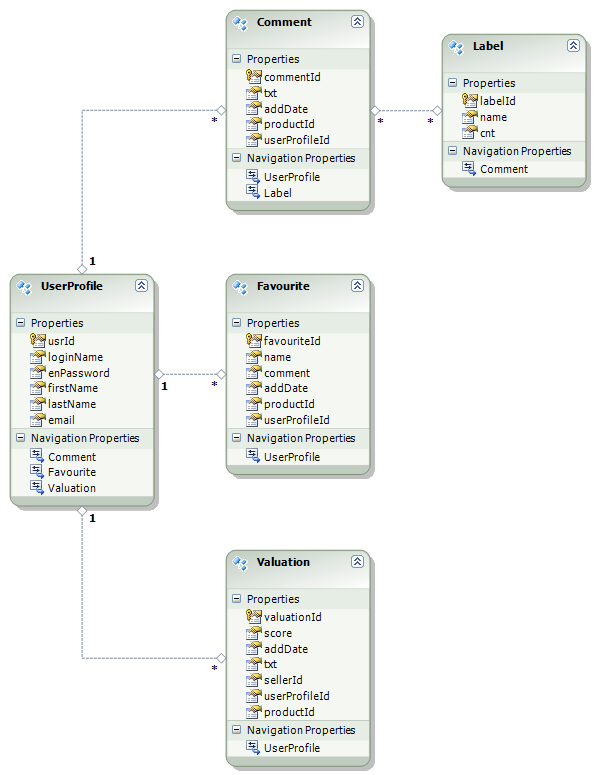
\includegraphics[width=0.75\textwidth]{img/EntityDesignerDiagram.png}
  \caption{Diagrama de clases persistentes.}
  \label{fig:ClasesPersistentes}
\end{figure}	
	
	
\subsection{Interfaces de los servicios ofrecidos por el modelo}

	El criterio que se ha seguido a la hora de diseñar las interfaces de los servicios ha sido el de agrupar por funcionalidades relacionadas. Los criterios para agrupar los casos de uso son los siguientes: aquellos relacionados con la búsqueda de productos \emph{ProductService}, la gestión los productos favoritos \emph{FavouriteService}, los referentes a operaciones propias de un usuario en \emph{UserService} y finalmente el resto de operaciones ofrecidas para tratar los comentarios así como las etiquetas de los mismos se agrupan en \emph{CommentService}.
	
	En la figura \ref{fig:ServiciosModelo} se muestran las fachadas (interfaces de los servicios) ofrecidos por el modelo con la declaración completa de sus operaciones y los tipos de dato que utilizan.

\begin{figure}[h]
  \centering
    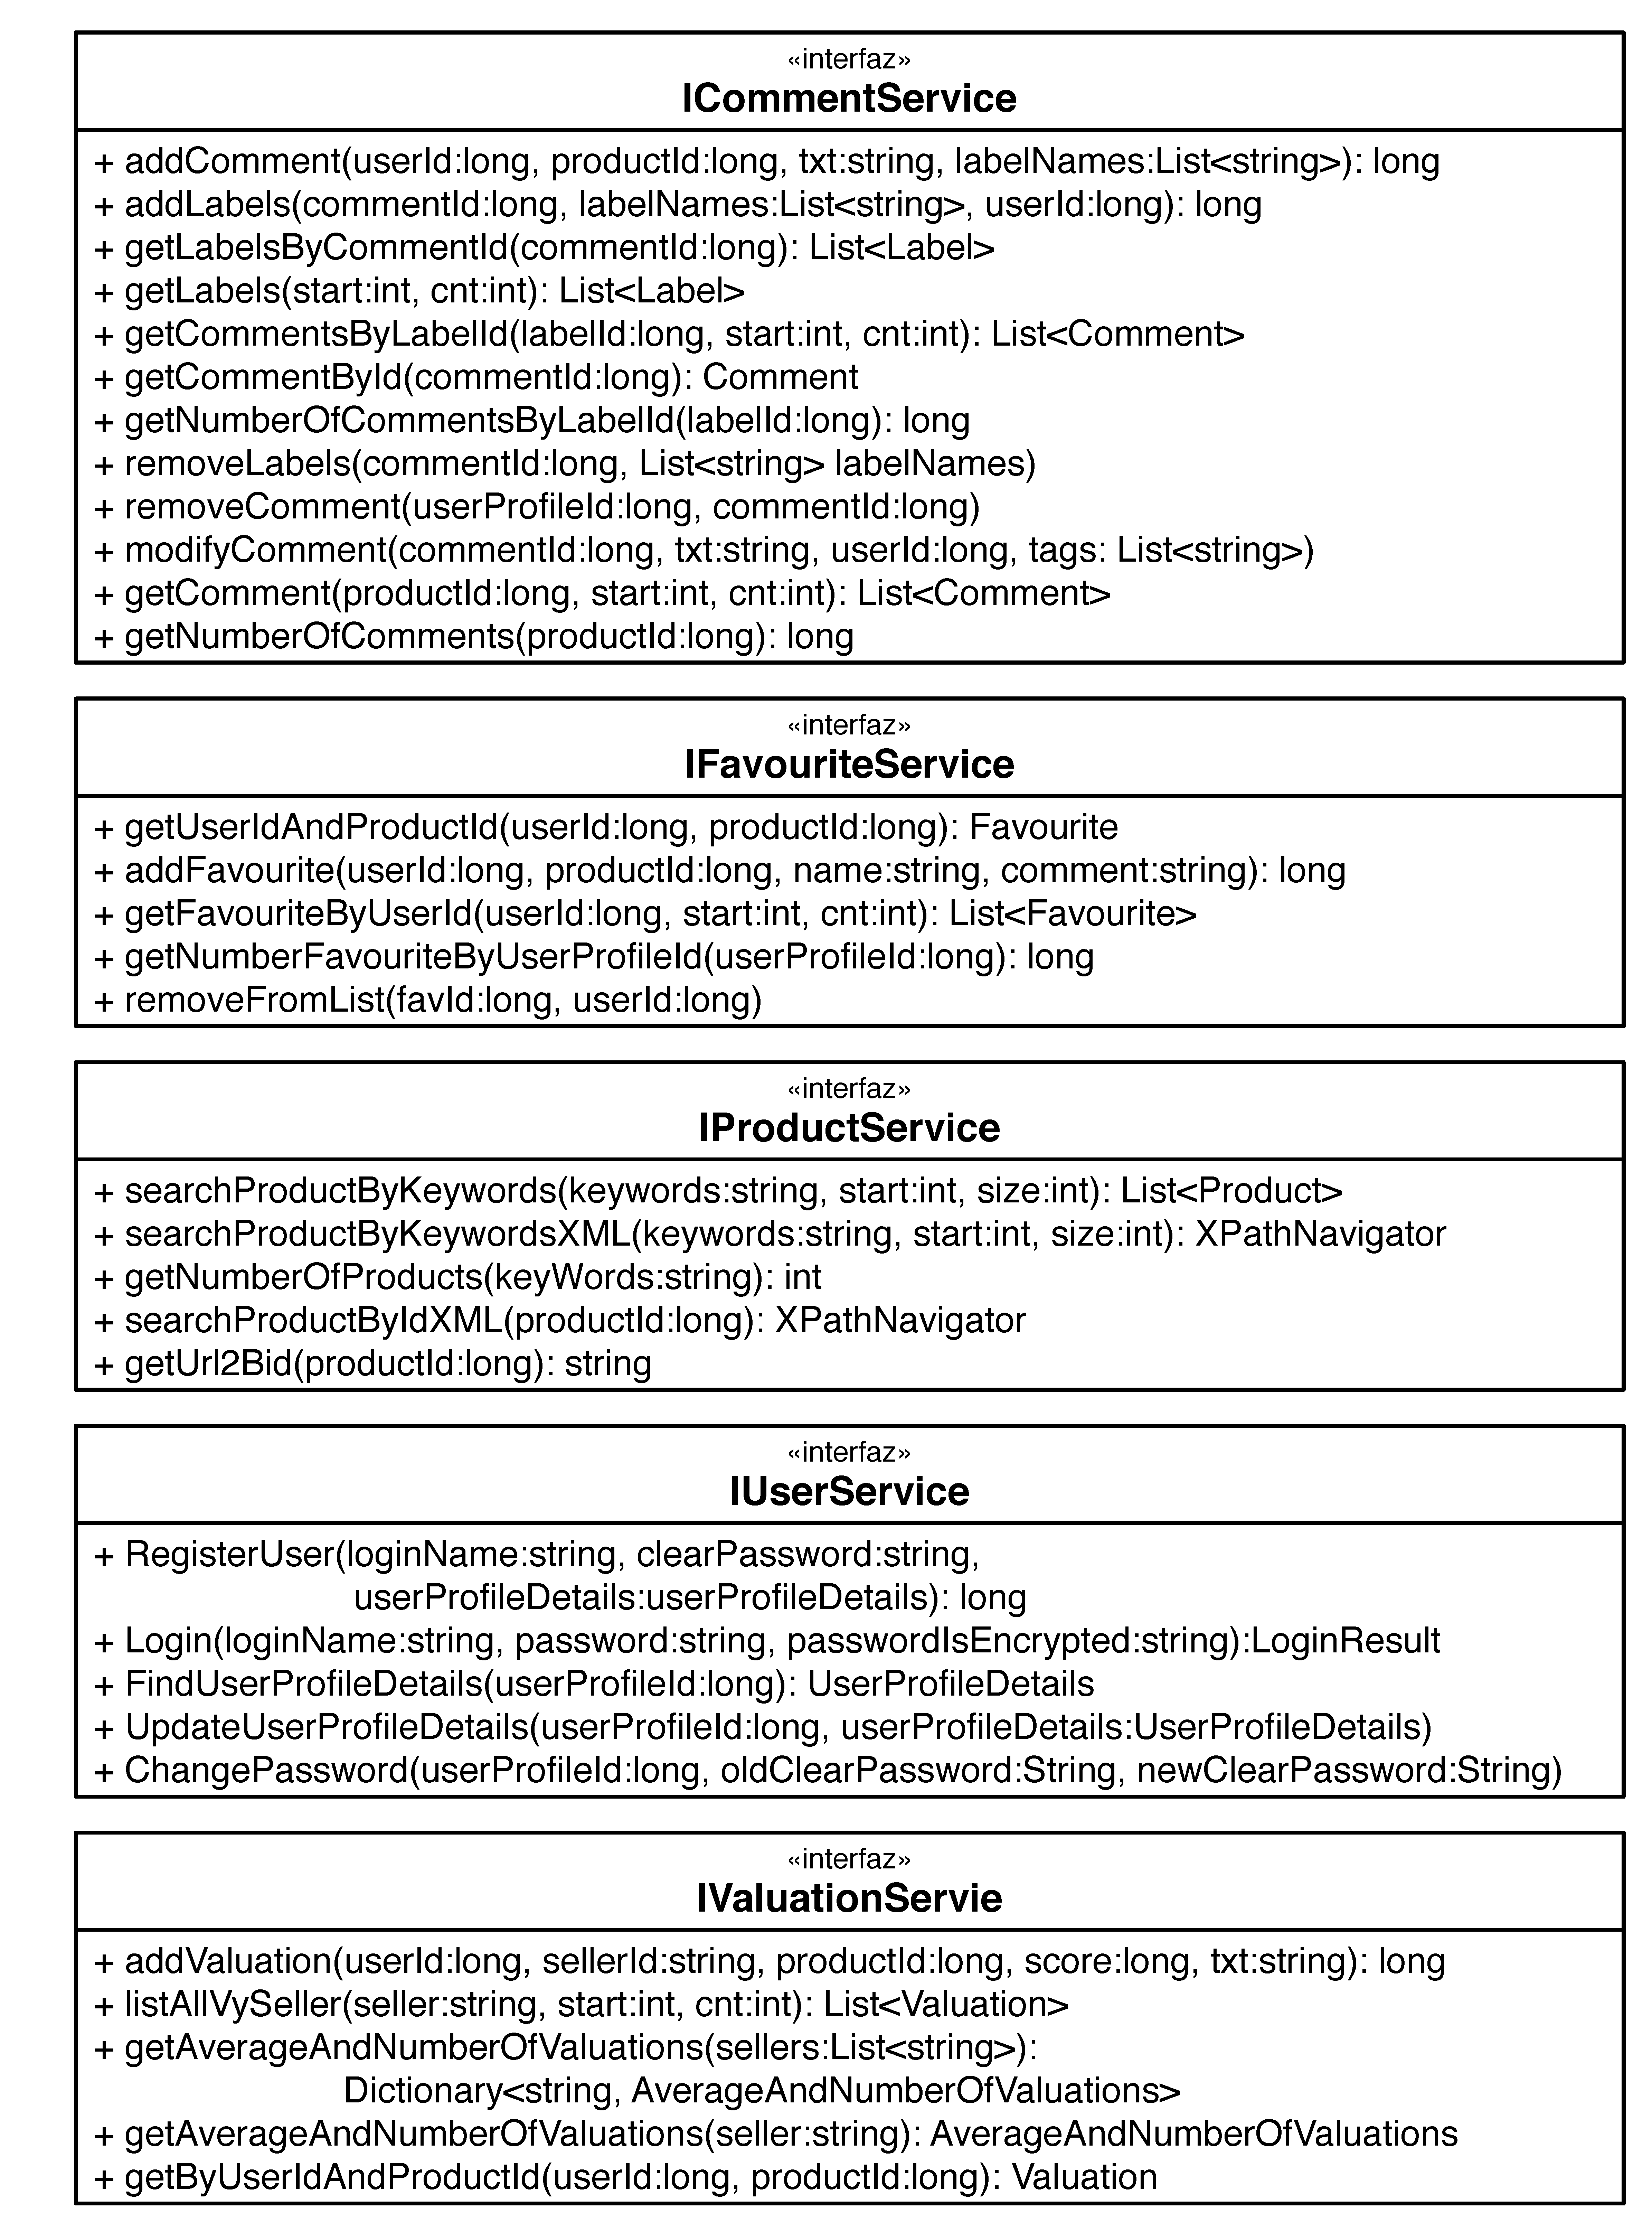
\includegraphics[width=0.75\textwidth]{img/servicios.pdf}
  \caption{Interfaces de los servicios ofrecidos por el modelo.}
  \label{fig:ServiciosModelo}
\end{figure}	

\subsection{Diseño de un DAO}

	A continuación, se presenta un diagrama de clases que ilustra la implementación de uno de los DAOs de la aplicación (concretamente, del DAO de la entidad \emph{Comment}) \footnote{No se muestra el diseño del resto de DAOs, dado que su arquitectura es similar.}.
	
\begin{figure}[h]
  \centering
    \includegraphics[width=0.85\textwidth]{img/CommentDao.pdf}
  \caption{Diagrama de clases del DAO de la entidad \emph{Comment}.}
  \label{fig:CommentDao}
\end{figure}	

\subsection{Diseño de un servicio del modelo}


	En este apartado se presenta un diagrama de clases con la implementación de un servicio del modelo, mostrando las dependencias con los DAOs que utiliza. Se ha elegido el servicio CommentService, puesto que se considera el más representativo y de mayor relevancia para la aplicación (en el sentido de que se trata de un sitio web de comentarios) \footnote{Al igual que en el apartado anterior (correspondiente a los DAOs) tampoco se muestra el diseño del resto de servicios, dado que su arquitectura es similar.}.

\begin{figure}[h]
  \centering
    \includegraphics[width=0.85\textwidth]{img/CommentService.pdf}
  \caption{Diagrama de clases del servicio ofrecido por \emph{CommentService}.}
  \label{fig:CommentService}
\end{figure}		
\clearpage

\subsubsection{Diagrama de secuencia: Añadir comentario a un producto} \label{cap:sec:model}

	En este apartado se expone un ejemplo de caso de uso que muestra la ejecución en la capa modelo. El caso de uso elegido ha sido el de 
	\emph{Añadir un comentario a un producto}, pues se considera representativo para la aplicación diseñada. A continuación se detallan los pasos 
	realizados en este caso de uso (véase el diagrama de secuencia presentado a continuación para seguir los pasos en ejecución de este caso de uso con mayor facilidad).
	
\begin{figure}[h]
  \centering
    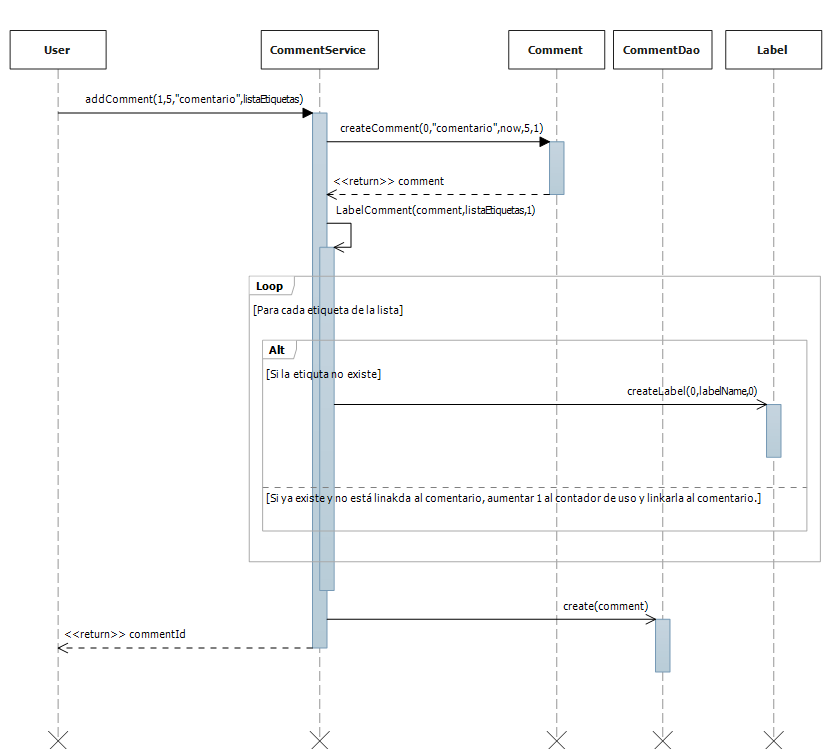
\includegraphics[width=0.9\textwidth]{img/AddCommentLabel.png}
  \caption{Diagrama de secuenta. Añadir un comentario.}
  \label{fig:AddCommentLabel}
\end{figure}		

\subsection{Otros aspectos}
	En este apartado se documentan algunos aspectos particulares que se consideran relevantes para la correcta comprensión de la capa modelo diseñada.
	
\subsubsection{Clases a medida}
	En algunos casos, en la capa web se requiere mostrar datos de más de una entidad. Devolviendo los objetos recuperados con \emph{Entity Framework}, se recuperan los objetos correspondientes al resto de asociaciones realizando consultas adicionales contra la base de datos para cada vez que se requiere datos que estén asociados a la relación.
	
	Para evitar esto, se pueden crear clases a medida que permiten obtener en una única consulta contra la base de datos la información necesaria de varias entidades.
	
	Como apunte, cabe indicar que, como las entidades no poseen datos muy voluminosos se incluyen los datos de las entidades asociadas mediante \emph{Include(``EntidadAsociada'')} para todos aquellos servicios que necesitan conocer algún valor de la relación de un objeto.
	
	La única ``clase'' a medida es \emph{AverageAndNumberOfValuations} que es una estructura para almacenar la puntuación de un vendedor y el número total de valoraciones que recibió hasta la fecha.

\subsubsection{Caché de contadores}
	Se ha implementado contadores caché para evitar el uso de la sentencia \emph{Count} contra la base de datos. De esta forma, cuando se necesite conocer el número total de datos asociados a una entidad, se recupera a través de un atributo que hace de contador incluido en la propia entidad.
	
	El uso de esta caché se ha empleado en la entidad \emph{Label} para poder conocer de antemano el número total de comentarios por cada etiqueta. Esto implica tener que realizar los controles necesarios desde \emph{CommentService} en los métodos que añaden y eliminan etiquetas asociadas a comentarios.
	
\subsubsection{Servicios XML}
	Para obtener los productos del servicio REST ofrecido por la aplicación web de subastas desarrollado en la primera parte de la asignatura, se añaden varios métodos en el servicio de productos dentro de la capa modelo. Concretamente dos métodos para obtener los ficheros XML con los datos de los productos, uno para la búsqueda de productos por palabras clave y otro para conocer los detalles de un producto concreto.
	
	A continuación se detallan los métodos del servicio \emph{ProductService}:
\begin{lstlisting}[style=sharpc]
 List<Product> searchProductByKeywords(string keywords, int start, int size);
\end{lstlisting}
	Recupera el listado de los productos \emph{XML} y lo parsea utilizando \emph{XmlDocument}.
\begin{lstlisting}[style=sharpc]
 XPathNavigator searchProductByKeywordsXML(string keywords, int start, int size);
\end{lstlisting}
	Devuelve un \emph{XML} de tipo \emph{XmlDocument} con el listado de los productos seleccionados a partir de una lista de palabras clave.
\begin{lstlisting}[style=sharpc]
 int getNumberOfProducts(string keywords);
\end{lstlisting}
	Recupera a partir del \emph{XML} el número total de productos. 
\begin{lstlisting}[style=sharpc]
 XPathNavigator searchProductByIdXML(long productId);
\end{lstlisting}
	Devuelve un \emph{XML} de tipo \emph{XmlDocument} con los detalles de un producto concreto.
\begin{lstlisting}[style=sharpc]
 string getUrl2Bid(int productId);
\end{lstlisting}
	Devuelve la url con la que se puede pujar por un producto.
	

\section{Interfaz gráfica}
	En esta sección se muestran los detalles de diseño e implementación de la capa vista de la aplicación.

\subsection{Diagrama de secuencia: Añadir comentario a un producto}
	En este apartado se expone un ejemplo de caso de uso que muestra su ejecución en la capa vista. El caso de uso elegido ha sido el de \emph{Añadir comentario a producto}
\footnote{Recuérdese que en un apartado previo \ref{cap:sec:model} se presentó el diagrama de secuencia en la capa modelo de este mismo caso de uso, lo cual permitirá obtener una visión completa de la ejecución de dicho caso de uso}
, pues se considera representativo para la aplicación diseñada. A continuación se detallan los pasos realizados en este caso de uso (véase el diagrama de secuencia presentado a en la figura \ref{fig:AddCommentLabelUI} para seguir los pasos en la ejecución de este caso de uso con mayor facilidad).

\begin{figure}[h]
  \centering
    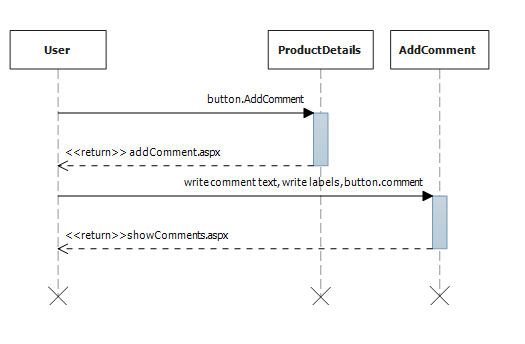
\includegraphics{img/AddCommentLabelUI.png}
  \caption{Diagrama de secuenta. Añadir un comentario.}
  \label{fig:AddCommentLabelUI}
\end{figure}		
	

\subsection{Otros aspectos.}
	En esta sección se documentan los aspectos particulares que se consideran relevantes para la correcta comprensión de la capa web.
	
\subsubsection{Control \emph{GridView}}
	El control \emph{GridView} ofrece la posibilidad de listar los datos en formato tabla y soportando múltiples opciones como la posibilidad de control de eventos por fila y edición de los datos.
	
	Para la paginación en los \emph{GridView} se ha implementado un método que devuelve los enlaces anterior y siguiente y un par de páginas próximas a la actual. Aunque el \emph{PagedDataSource} es implementado por los \emph{GridView} se ha decidido no emplearlo por su complejidad y la opción de los enlaces permite seleccionar sólo los datos necesarios en cada petición de una forma muy simple.
	
	Para realizar la personalización del listado se añade la llamada a la función en el \emph{GridView}  {\color{red} OnRowDataBound}{\color{blue}=''DataBoundRecord''}. La función en el \emph{Code-Begind} que realiza las siguientes comprobaciones se muestra a continuación.	

\begin{lstlisting}[style=sharpc]
protected void DataBoundRecord(object sender, GridViewRowEventArgs e)
{
	if (e.Row.RowType == DataControlRowType.DataRow)
	{
		HyperLink linkMod = (HyperLink)e.Row.FindControl("lnkButtonModify");
		LinkButton linkDel = (LinkButton)e.Row.FindControl("lnkButtonDelete");
		Comment comment = (Comment)e.Row.DataItem;

		linkMod.NavigateUrl = String.Format("~/Pages/Product/AddComment.aspx?comment={0}&id={1}", comment.commentId,id);

		if (userId != comment.userProfileId)
		{
			linkDel.Visible = false;
			linkMod.Visible = false;
		}
	}

}
\end{lstlisting}

	También es posible crear \emph{GridView} que soporten las operaciones \emph{CRUD}. Un ejemplo donde se puede ver el uso de este tipo de \emph{GridView} se puede ver en el manejo de favoritos, donde un usuario puede eliminar un producto de su lista de deseos. En este caso de eliminación se se puede personalizar una columna con \emph{TemplateField}. Así es posible por ejemplo definir la acción de un control. A continuación se muestra este ejemplo de eliminar un producto de la lista de favoritos del \emph{GridView}:

\begin{lstlisting}[style=xml]
<asp:TemplateField>
	<ItemTemplate>
		<asp:LinkButton ID="lnkButton" runat="server"
		    commandName="Delete" CssClass="btn btn-danger"
		    OnClientClick=<%# String.Format("return confirm('{0}');", GetLocalResourcesObject("Comfirm_Delete")) %>
			
			<span class="icon-trash icon-white">
		    </span>
		    &#160;
		    <asp:Localize ID="lclDelete" runat="server"
		    	    Text="<%$ Resources:Common, Delete %>" />
		</asp:LinkButton>
	</ItemTemplate>
</asp:TemplateField>
\end{lstlisting}

	La opción \emph{OnClientClick} realiza una petición de javascript sobre el navegador del cliente solicitando una confirmación con el texto del recurso global \emph{PONER AQUI LA CLAVE DEL ARCHIVO DE I18N}.
	
	La opción \emph{CommandName} define que tipo de acción implica el enlace definido.
	
	Finalmente, el método del evento en el dato servidor se define en un atributo del elemento \emph{GridView}:  {\color{red} OnRowDeleting}{\color{blue}=''DeleteRecord''} junto con el identificador del producto que va a eliminar {\color{red} DataKeyNames}{\color{blue}=''favouriteId''}.
	
	En el método \emph{DeleteRecord} se obtiene el identificador a partir del objeto {\color{BlueGreen} GridViewDeleteEventArgs}
	
	Con el identificador devuelto se realiza la llamada al método del servicio y finalmente se recargan los nuevos datos en el \emph{GridView}.
	
\subsubsection{XSLT}
	Los servicios web de productos a partir de ficheros \emph{XML} remoto son procesados por el traductor \emph{XSLT} que ayuda a la transfomación de \emph{XML} facilitando su presentación en las páginas \emph{ASP.NET}.
	
\textbf{Tranformación \textit{XSLT} del listado de productos.}
	
	El \emph{XML} del listado de productos se procesa y se transforma en una tabla \emph{HTML}.
	
	Para obtener los productos se obtiene una única regla que recupera los nodos \emph{product} a partir del nodo raíz \emph{products}. Cada nodo \emph{product} contiene lso atributos de nombre, categoría, precio y tiempo que resta para que finalice la subasta, el subastador entre otros.
	
	
\textbf{Transformación \textit{XSLT} de los detalles de un producto.}

	El \emph{XML} de los detalles de producto es procesado y transformado en una tabla de \emph{HTML}. Al igual que antes existe un elemento raíz \emph{products} que en este caso solo contendrá un único elemento
\footnote{En el caso de que se busque un producto que no exista se devolverá el nodo raíz \emph{products} sin ningún nodo hijo.}	
\emph{product} que contiene los detalles del producto en sus atributos.

\textbf{Internacionalización en el fichero \textit{XSLT}.}

	Para añadir \emph{i18n} se añaden los valores de los recursos globales como parámetros al \emph{XSLT} desde el \emph{Code-Behind} de las páginas con \emph{XsltArgumentList}.
	
\textbf{Paginado.}

	También se contempla la paginación en el listado de los productos. Para ello se hace uso del atributo \emph{total} que está en el nodo raíz (\emph{products}) del fichero \emph{XML} que indica el número de productos que cumplen el criterio de búsqueda especificado.
	
	Gracias a ese atributo, podemos tener una paginación igual que la que se obtiene mediante el \emph{GridView}.

\section{Funcionalidad adicional}
	
	En este apartado se explica cómo se ha realizado cada parte adicional.	
	
\subsection{Parsing de XML}

	Se incorpora al formulario de búsqueda de productos la opción de especificar si la búsqueda debe incluir la información sobre los votos que recibió o no. Cuando un usuario especifica que se incluya información de los votos en el resultado de la búsqueda, por cada usuario que aparezca se mostrará adicionalmente el número de votos realizados sobre él.
	
	El número de valoraciones sólo se mostrará si existen valoraciones para ese vendedor en concreto. Su implementación se explica en los siguientes apartados.
	
\subsubsection{Capa modelo}
	Para la implementación del parsing \emph{XML} se incluye el método \emph{searchProductByKeywords}. Se realiza la búsqueda de productos con la clase \emph{XmlDocument} y el método \emph{GetElementsByTagName} con el que se obtiene una lista de nodos \emph{XmlNodeList}.
	Por cada nodo se crea un objeto de tipo Product, el cual contiene nombre, vendedor, categoría, precio y minutos para finalizar la subasta. Durante la creación se realizan las siguientes operaciones:
\begin{itemize}
	\item El identificador de cada subastador se obtiene a partir del fichero \emph{XML}.
	\item El número total de valoraciones se obtiene de la propia aplicación haciendo uso del servicio \emph{ValuationService} con el método \emph{getAverageAndNumberOfValuations} que recibe por parámetro el identificador de cada vendedor.
\end{itemize}
	
	Para poder realizar el paginado se añade al servicio el método \emph{getNumberOfProducts} que comprueba en el archivo \emph{XML} (usando \emph{XmlDocument} y \emph{XPath}) si existe el atributo \emph{total} dentro de la etiqueta \emph{products}.

\subsubsection{Capa web}
	En la página \emph{aspx} se muestra la información de los productos a través de un 
\emph{Repeater} en lugar de usar el XSLT.
	Los enlaces para añadir comentario, añadir favorito y valorar incluyen un parámetro en la URL con el identificador del producto mientras que el enlace de ver valoraciones incluye el usuario del vendedor en la URL.
\subsection{Etiquetado de comentarios}

	En este apartado se especifica la funcionalidad de etiquetado de comentarios. En el momento de añadir un comentario el usuario podrá añadir una 
	serie de etiquetas. Se podrán utilizar etiquetas ya existentes o incluir etiquetas nuevas. La aplicación es capaz de controlar, a través de los 
	servicios de la capa modelo, si una etiqueta existe o debe crearse. Además, para cada comentario se realiza la comprobación de que la etiqueta no 
	esté ya añadida al mismo. Para los comentarios ya etiquetados, se podrá ``desetiquetar'' una o varias etiquetas ya asociadas y también se permitirá
	añadir nuevas etiquetas.\\
	
	Las etiquetas se pueden añadir en el momento de crear un comentario. Deben ir separadas por comas y pueden incluír espacios en blanco. Es posible
	añadir un comentario sin asignarle etiquetas, pudiendo asignárselas más tarde a través del botón ``modificar'' en la lista de comentarios. \\Cuando
	se pulsa este botón, en la página a la que redirige, se cargan los datos que había previamente, tanto el texto del comentario como el de las etiquetas,
	en caso de que exista. Si se desean añadir más etiquetas, basta con seguir añadiéndolas, separadas por comas, a las ya existentes. Si se quieren
	eliminar de ese comentario, lo único que hay que hacer es borrar el texto de las etiquetas que ya no se quieran. Al pulsar el botón ``comentar'' se
	actualizarán las etiquetas ligadas a ese comentario.
	
\subsubsection{Contador caché en etiquetas}

	Para evitar peticiones pesadas contra el SGBD, se implementa un contador caché sobre la entidad \emph{Label}, el cual contabiliza el número de veces que aparece una etiqueta en los comentarios. Es en la propia implementación del servicio (\emph{CommentService}) donde se tiene en cuenta el incremento o decremento del contador cuando se agrega o elimina una etiqueta concreta de un grupo de usuarios.

\section{Compilación e instalación de la aplicación}

	En este apartado se explica cómo compilar e instalar la aplicación, asumiendo un entorno correctamente configurado.
	
	En primer lugar, se debe configurar y crear la base de datos desde \emph{Visual Studio 2010} con la solución del proyecto abierta. A continuación se condiguran los ficheros necesarios para el acceso y los valores de los datos de acceso al servidor de aplicaciones \emph{Tomcat}. Estos pasos se detallan en la siguiente lista:
\begin{enumerate}
	\item Crear la base de datos desde \emph{Server Explorer} $\rightarrow$ \emph{Data conections} $\rightarrow$ \emph{Create New SQL Server Database}$\ldots$. En la ventana seleccionar el nombre del servidor \emph{``localhost\textbackslash SQLExpress''}.
	
	\item Ir al proyecto \emph{Model} y en la carpeta \emph{Sql} abrir \emph{SqlServerCreateTables.sql} y sobre el dicho archivo pulsar con el botón derecho del ratón y seleccionar \emph{Execute SQL}. Lo que hará sera ejecutar el script sobre la base de datos PrácticaIS.
	
	\item Modificar el nombre del esquema de usuario de la base de datos en el proyecto \emph{Model} $\rightarrow$ \emph{MiniPortalEntityDataModel.edmx}. En el ejemplo, el esquema de usuario de BBDD es \emph{dbo}.
\begin{lstlisting}[style=xml]
<EntitySet Name="Comment" EntityType="Es.Udc.DotNet.MiniPortal.Model.Store.Comment" store:Type="Tables" Schema="dbo" />
<EntitySet Name="Favourite" EntityType="Es.Udc.DotNet.MiniPortal.Model.Store.Favourite" store:Type="Tables" Schema="dbo" />
<EntitySet Name="Label" EntityType="Es.Udc.DotNet.MiniPortal.Model.Store.Label" store:Type="Tables" Schema="dbo" />
<EntitySet Name="LabelComment" EntityType="Es.Udc.DotNet.MiniPortal.Model.Store.LabelComment" store:Type="Tables" Schema="dbo" />
<EntitySet Name="UserProfile" EntityType="Es.Udc.DotNet.MiniPortal.Model.Store.UserProfile" store:Type="Tables" Schema="dbo" />
<EntitySet Name="Valuation" EntityType="Es.Udc.DotNet.MiniPortal.Model.Store.Valuation" store:Type="Tables" Schema="dbo" />
\end{lstlisting}

	\item Modificar el nombre de la conexión a la base de datos en el proyecto \emph{Model} $\rightarrow$ \emph{App.config}, el proyecto \emph{Test} $\rightarrow$ \emph{App.config} y en el proyecto \emph{Web} $\rightarrow$ \emph{Web.config}.
\begin{lstlisting}[style=xml]
<connectionStrings>
    <add name="MiniPortalEntitiesContainer"
         connectionString="metadata=res://*/MiniPortalEntityDataModel.csdl|res://*/MiniPortalEntityDataModel.ssdl|res://*/MiniPortalEntityDataModel.msl;provider=System.Data.SqlClient;provider connection string=&quot;data source=localhost\SQLExpress;initial catalog=PracticaIS;integrated security=True;multipleactiveresultsets=True;App=EntityFramework&quot;"
         providerName="System.Data.EntityClient" />

</connectionStrings>
\end{lstlisting}

	\item Añadir los parámetros para el acceso al servicio web de subastas. Dentro de las propiedades del proyecto \emph{Model} (botón derecho sobre el proyecto y la opción \emph{Settings}) se debe configurar los parámetros de los servicios y páginas \emph{XML}, además de los parámetros de búsqueda:
	\begin{itemize}
		\item \textbf{XmlRemoteHost}: Especifica el servidor web remoto.
		\item \textbf{XmlProductList}: Especifica la ruta hacia el servicio \emph{REST} de búsqueda de productos.
		\item \textbf{XmlProduct}: Especifica la ruta hacia el servicio \emph{REST} para conocer los detalles de un producto.
		\item \textbf{BidRemoteHost}: Especifica la ruta hacia la puja de un producto.
		\item \textbf{DefaultPageSize}: Valor de elementos que se deben de recuperar en caso de que no se reciba un valor específico.
	\end{itemize}

	\item Seleccionar el proyecto \emph{Web} como proyecto de inicio (seleccionamos el proyecto y con el botón derecho del ratón se selecciona la opción \emph{Set as StartUp Project}).
	
	\item Seleccionar la página principal en el proyecto \emph{Web} $\rightarrow$ \emph{Pages} $\rightarrow$ \emph{MainPage.aspx} (click con el botón derecho sobre el archivo y seleccionar \emph{Set as Start Page}).
	
	\item Finalmente, para su ejecución en desarrollo pulsar \emph{Control + F5} lo que iniciará el servidor por defecto y accederá a la página de inicio del proyecto web.
\end{enumerate}

%\section{Problemas conocidos}

\clearpage
%%%%%%%%%%%%%%%%%%%%%%%%%%%%%%%%%%%%%%%
%%%%%%%%%%%%%%%%%%%%%%%%%%%%%%%%%%%%%%%
%% Para la parte final del documento %%
%%%%%%%%%%%%%%%%%%%%%%%%%%%%%%%%%%%%%%%
%%%%%%%%%%%%%%%%%%%%%%%%%%%%%%%%%%%%%%%
\newpage
\listoffigures

\end{document}